\section{Modelos de Estructura Urbana e Interacción}

\begin{frame}{Modelos de Estructura Urbana en la ZMVM}
  \begin{columns}[c]
    % --- COLUMNA IZQUIERDA: EXPLICACIÓN COMPLEMENTARIA ---
    \begin{column}{0.40\textwidth}
      \begin{itemize}
        \item \scriptsize \textbf{Anillos:} Crecimiento radial desde el núcleo central hacia periferias residenciales.
        \item \scriptsize \textbf{Sectores:} Formación de cuñas siguiendo ejes de transporte; ej. Corredor 
                \textit{Reforma-Santa Fe} (lujo) e \textit{Industrial Vallejo} (norte).
        \item \scriptsize \textbf{Núcleos:} La CDMX como múltiples polos independientes como 
                \textit{Satélite, Polanco, CU y Santa Fe} \cite{padilla2022expansion}.
      \end{itemize}
      
      \vspace{0.3cm}
      
      \begin{exampleblock}{\footnotesize Análisis Topológico}
        \tiny Esta estructura de núcleos genera un mosaico de retículas desfasadas que requiere integración \cite{garibaldi2023vft}.
      \end{exampleblock}
    \end{column}
    \begin{column}{0.58\textwidth}
      \begin{figure}
        \centering
        
\includegraphics[width=\textwidth, height=0.75\textheight, keepaspectratio]{ArichieExpress.JPEG}
        \caption{\scriptsize Esquema de nodos y flujos (Archie's Press).}
      \end{figure}
    \end{column}
  \end{columns}
\end{frame}

\begin{frame}{Comparativa de Movilidad: CDMX vs. Estado de México}
  \begin{columns}[c]
    % --- COLUMNA IZQUIERDA: DATOS ---
    \begin{column}{0.52\textwidth}
      \begin{block}{\footnotesize Dinámicas de Traslado (2020)}
        \centering
        \scriptsize
        \begin{tabular}{lcc}
          \toprule
          \textbf{Indicador} & \textbf{CDMX} & \textbf{Edomex} \\
          \midrule
          Tiempo trab. (min) & 43.4 & 45.5 \\
          Viajes > 1h (trab.) & 20.2\% & 24.2\% \\
          Tiempo col. (min) & 27.3 & 22.6 \\
          \midrule
          Medio Trabajo & Particular & Caminando \\
          Medio Estudios & Público & Público \\
          \bottomrule
        \end{tabular}
      \end{block}
      \vspace{-0.2cm}
      \begin{alertblock}{\tiny Análisis de Dependencia}
        \tiny El 24.2\% del Edomex invierte >1h al empleo, reflejando la segregación de las \textit{periferias dormitorio} \cite{dataMexicoEdomex}.
      \end{alertblock}
    \end{column}
    \begin{column}{0.45\textwidth}
      \begin{figure}
        \centering
        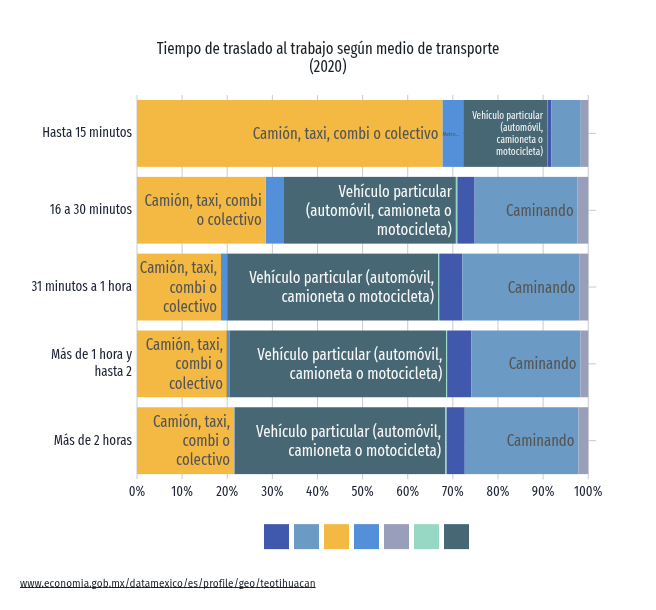
\includegraphics[width=0.7\textwidth, height=0.35\textheight, keepaspectratio]{img/TiempoTrasladoCDMX.png}
        \vspace{0.1cm}
        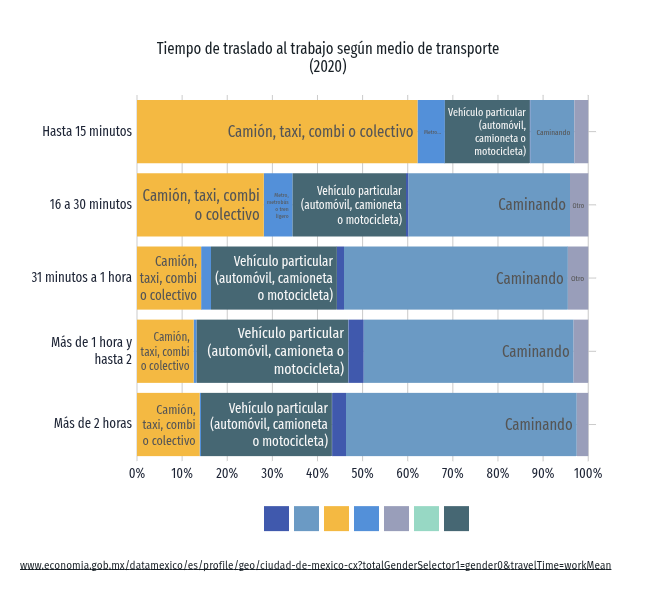
\includegraphics[width=0.7\textwidth, height=0.35\textheight, keepaspectratio]{img/TiempoTrasladoEDOMEX.png}
        \caption{\tiny Estructura de viajes: CDMX (Izquierda) \cite{dataMexicoCDMX} vs Edomex (Derecha) \cite{dataMexicoEdomex}.}
      \end{figure}
    \end{column}
  \end{columns}
\end{frame}
